% Template Created by Mau Muñoz (https://github.com/maumchaves) following the specification for thesis documents provided by the Universitat Pompeu Fabra, Barcelona (https://guiesbibtic.upf.edu/tesis/eng/writing).

\documentclass{upfthesis}

\usepackage[utf8]{inputenc}

% TL;DR: Times-New-Roman-like font for Latex
% https://ctan.org/pkg/mathptmx
\usepackage{mathptmx}

% Can be changed according to your requirements
\usepackage[english]{babel}
\selectlanguage{english}

\usepackage{graphicx}
\graphicspath{ {images/} }

\usepackage{subcaption}

\usepackage{csquotes}

% Generates random content to fill this template
\usepackage{blindtext}
\usepackage{lipsum}

% Only (useful) for testing
\usepackage{showframe}

% Required only to style code snippets
\usepackage{listings}
\usepackage{color}
\definecolor{codebackcolor}{rgb}{0.95,0.95,0.92}
\lstdefinestyle{codestyle}{
    backgroundcolor=\color{codebackcolor},
    basicstyle=\footnotesize\ttfamily,
    breakatwhitespace=false,
    breaklines=true,
    keepspaces=true,
    showspaces=false,
    showstringspaces=false,
    showtabs=false,                  
    tabsize=4
}
\lstset{style=codestyle}

\usepackage{hyperref}

\title{UPF Thesis Template in \LaTeX{}}
\author{Mau Muñoz}
\date{July 2019}
% To update the date at the time you compile your document
% \date{\today}

\begin{document}

\maketitle

\begin{abstract}
  This is a simple paragraph at the beginning of the document. A brief introduction about the main subject.
\end{abstract}
 
We have now added a title, author and date to our first \LaTeX{} document!

Some of the \textbf{greatest}
discoveries in \underline{science} 
were made by \textbf{\textit{accident}}.

This is an \emph{emphasized} word inside normal text. \textit{And this is an \emph{emphasized} word inside an italicized text.}

\textbf{Baseline image:}

\blindtext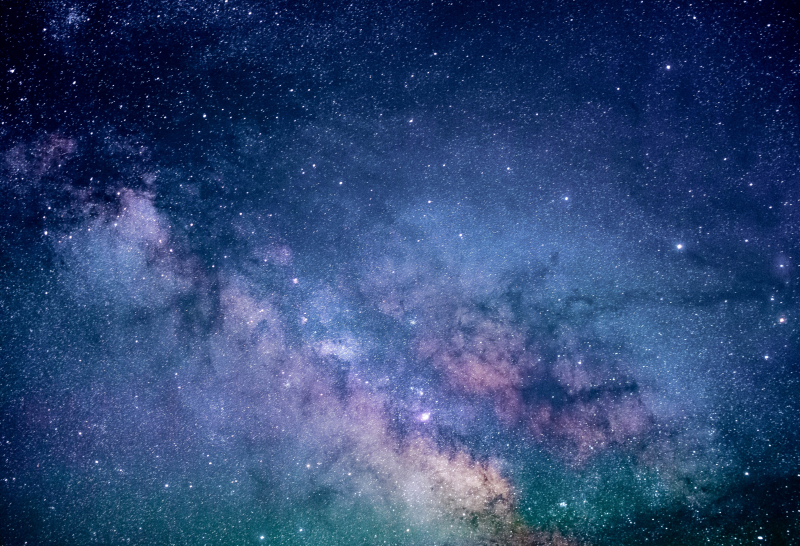
\includegraphics[height=\baselineskip]{image-1}.

\newpage

\textbf{Full width image:}
\\ % break line: starts a new line (also `\newline`).
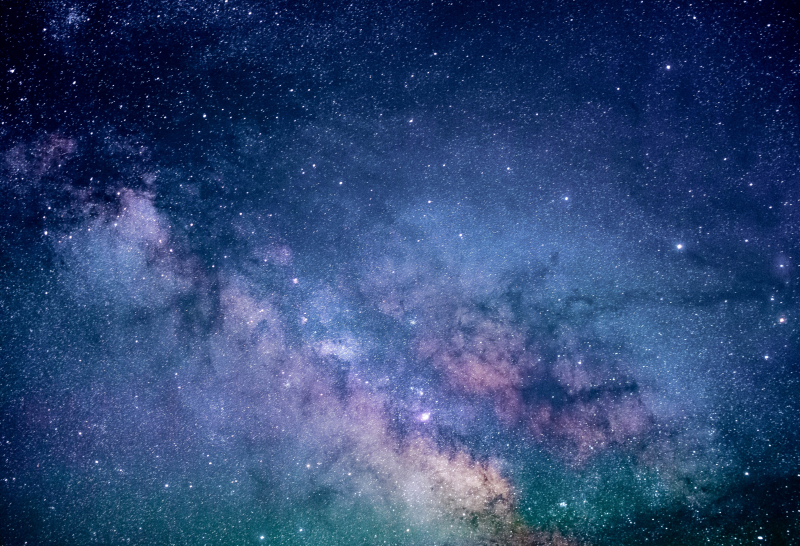
\includegraphics[width=\linewidth]{image-1}

\textbf{Image with max height:}
\\
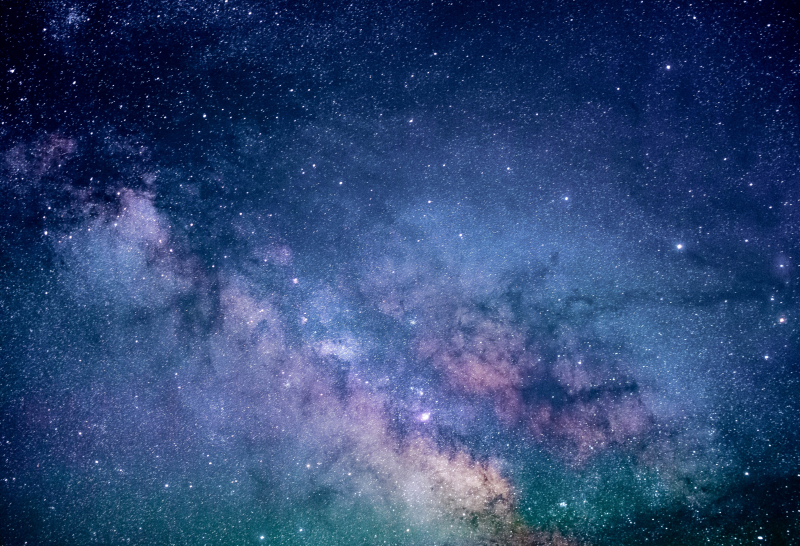
\includegraphics[height=3cm]{image-1}

\newpage

\textbf{Images in a grid:}
\\
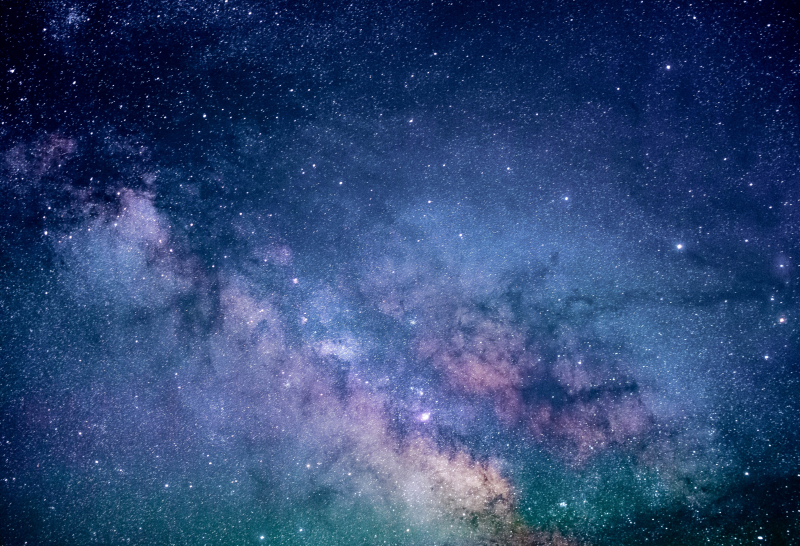
\includegraphics[width=.3\linewidth]{image-1}\quad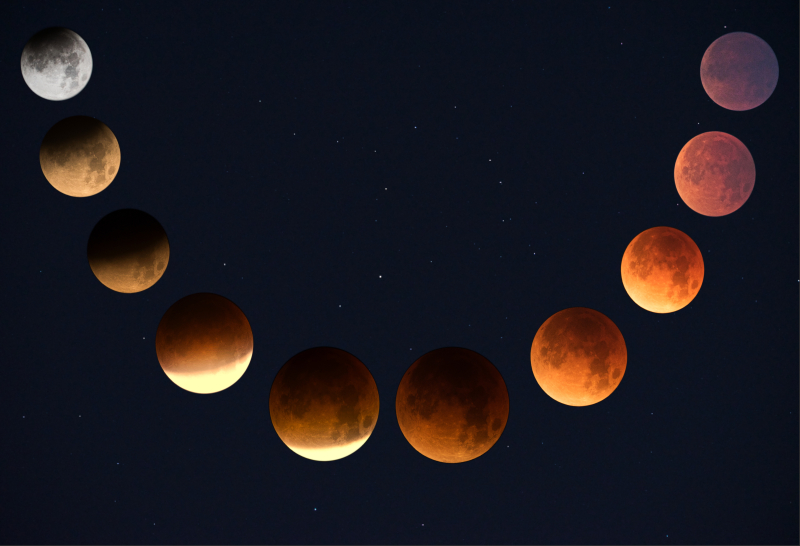
\includegraphics[width=.3\linewidth]{image-2}\quad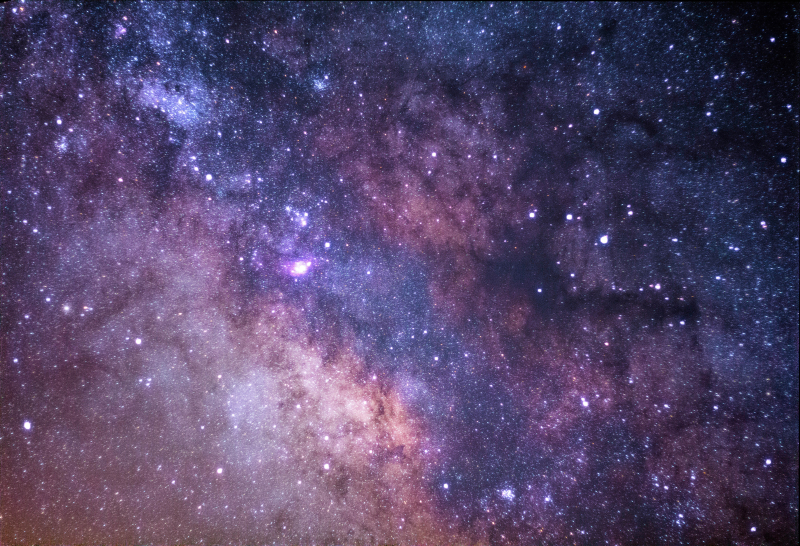
\includegraphics[width=.3\linewidth]{image-3}
\\[\baselineskip]% adds vertical line spacing
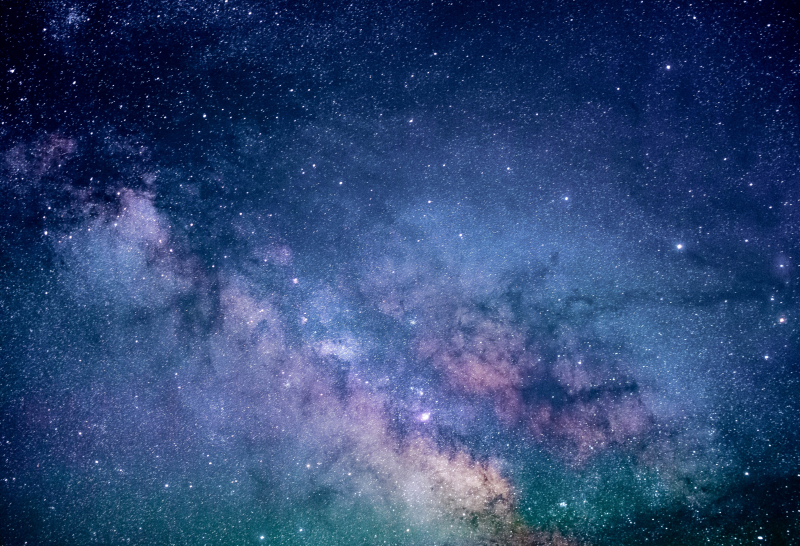
\includegraphics[width=.3\linewidth]{image-1}\quad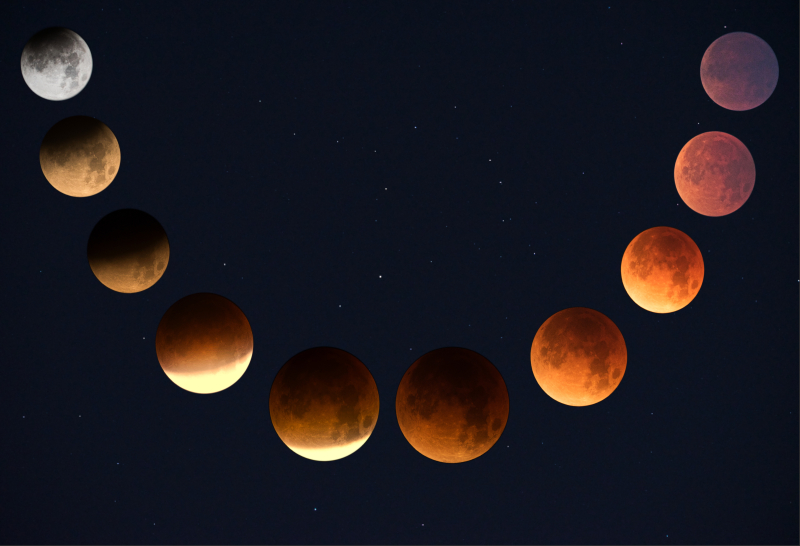
\includegraphics[width=.3\linewidth]{image-2}\quad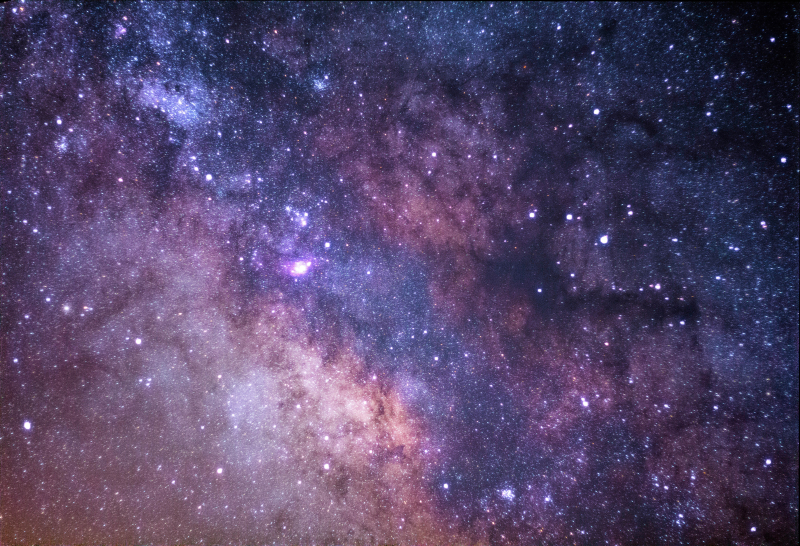
\includegraphics[width=.3\linewidth]{image-3}

\textbf{Centering image with caption:}
\\
\begin{figure}[h]
  \centering
  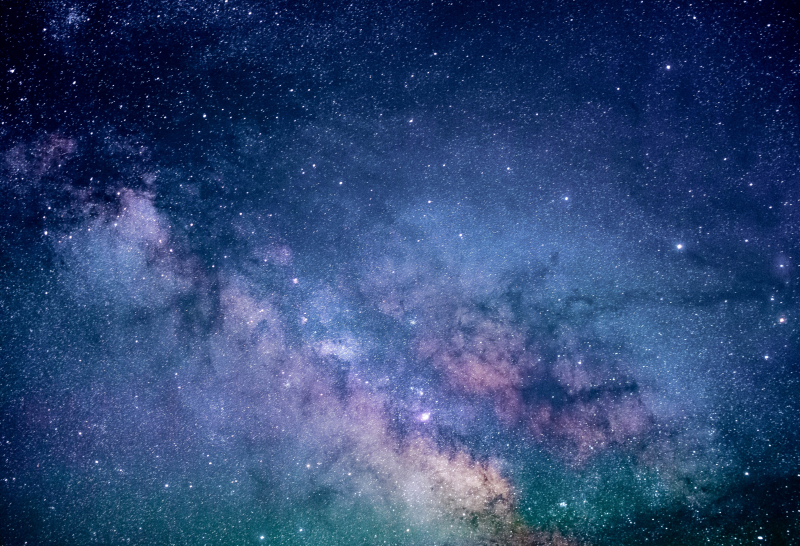
\includegraphics[width=0.5\textwidth]{image-1}
  \caption{a nice plot}
  \label{fig:image1}
\end{figure}

\textbf{Reference a figure:}

You can reference the figure \ref{fig:image1}. Also, you can reference the page \pageref{fig:image1} where the figure is.

\textbf{Unordered lists:}

\begin{itemize}
  \item The individual entries are indicated with a black dot, a so-called bullet.
  \item The text in the entries may be of any length.
\end{itemize}

\textbf{Ordered lists:}

\begin{enumerate}
  \item The individual entries are indicated with a black dot, a so-called bullet.
  \item The text in the entries may be of any length.
  \item \blindtext
\end{enumerate}

\textbf{Aligned text:}
\begin{center}
  Example 1: This text is an example of Center Alignment using the center environment. You can also use \verb|flushleft| and \verb|flushright|.
\end{center}

\textbf{New Paragraph:}
This is the text in first paragraph. This is the text in first paragraph. This is the text in first paragraph. \par
This is the text in second paragraph. This is the text in second paragraph. This is the text in second paragraph.

\end{document}